\documentclass[final,5p,times,twocolumn]{elsarticle}
\usepackage{amsmath,amssymb}
\usepackage{graphicx}
\usepackage{booktabs}
\usepackage{array}
\usepackage[hidelinks]{hyperref}

\journal{Future Generation Computer Systems}
\setlength{\emergencystretch}{2em}
\setlength{\bibsep}{0pt}
\newcolumntype{P}[1]{>{\raggedright\arraybackslash}p{#1}}

\begin{document}

\begin{frontmatter}

\title{From Semantics to Decisions: A Federated Vision-Language Decision Model for UAV Power-Line Inspection}

\author{Mahdi Khashan}
\ead{mahdikhashan1@gmail.com}
\affiliation{organization={[Affiliation to be added]}}

\begin{abstract}
A recent agenda for edge-native semantic UAV inspection shows that a lightweight vision-language model (VLM) runs on a Jetson-class drone computer at 2.8\,s per image, and leaves speed, measured reliability, training data and fleet collaboration open. We study a vision-language \emph{decision model}, laya-vision (201M parameters), which answers typed inspection questions in one forward pass with calibrated probabilities, not generated text. On 35,415 power-line component images (ElecVQA-Bench, InsPLAD), the published checkpoint fails zero-shot (condition macro F1 0.180). Fine-tuning on 4,807 images with labels from the dataset folders raises it to 0.703, with component accuracy 0.924 and defect AUROC 0.965, at 74\,ms per image for four questions on an RTX 2080 Ti. As a trigger, the defect probability passes 15.3\% of images on and finds 88.5\% of defects. With FedAvg over simulated tower-wise drones, accuracy falls as the data is split further (macro F1 0.624, 0.541, 0.474 for 3, 6, 18 drones) but stays above drones that train alone (0.371), and a start fine-tuned on separate server towers brings the fleet to 0.636. From the published checkpoint, small updates (17--45\,MB) learn little in ten rounds (macro F1 0.24--0.28), more rounds help (0.49 after 30), int8 updates cost nothing measurable and FedProx changes nothing. With 100--200 natural labels per drone, fleet FedAvg from the server model raises defect AUROC from 0.903 to 0.93, but 25--50 labels lower it and pooling is better (0.958). Drones that each see different components learn their own defect type alone, which small-update FedAvg loses for every split.
\end{abstract}

\begin{keyword}
semantic edge intelligence \sep vision-language model \sep decision model \sep federated learning \sep UAV inspection \sep power lines
\end{keyword}

\end{frontmatter}

\section{Introduction}

Farahani et al.~\cite{p2s} describe how inspection pipelines move from cloud-centric image analysis, through onboard detectors such as YOLO, to \emph{edge-native semantic inspection}, in which a lightweight vision-language model (VLM) on the drone interprets what the detector found. Their feasibility study on an NVIDIA Jetson Orin shows that this is possible but slow: a fine-tuned SmolVLM-256M~\cite{smolvlm} needs about 2.8\,s per image, against 0.14\,s for YOLO26M, and continuous captioning of a 10\,s, 30\,fps clip takes about 14\,min~\cite{p2s}. The same group's EVLM system~\cite{evlm} reports 1.4--6.4\,s per 4\,s video segment for a LoRA-tuned SmolVLM on power-line inspection, and a companion study profiles cloud, onboard and split deployment of such models~\cite{splitvlm}.

The agenda in~\cite{p2s} leaves several challenges open, five of which are the starting point of this paper: low-latency multimodal reasoning, hierarchical processing in which an inexpensive stage decides when the expensive VLM runs, training data without captions generated by GPT-4o, confidence estimates that a mission planner can act on, and collaborative training across many UAVs. Its feasibility study also shows semantic quality only with three qualitative examples.

Many inspection questions do not need free text. ``Does this clamp have a defect?'' and ``Which condition does this insulator have?'' are choices among known options. \emph{Decision models} answer such typed questions in one forward pass and return a probability for each option. Laya~\cite{laya} introduced the design for text, and laya-vision~\cite{layavision} replaces its text encoder with a truncated SmolVLM backbone, so that the input can be an image. A decision model is therefore a natural middle stage between a detector and a describing VLM: it keeps the vision-language backbone, but gives labels and probabilities at a cost close to one image encoding.

The images that would improve such a model are spread across the fleet that collected them. Different operators may own the drones, and imagery of critical infrastructure is sensitive. Federated learning~\cite{fedavg} trains one model across clients without moving their data, but inspection data differs strongly between drones, because each drone flies its own towers.

We ask how well such a decision model classifies power-line components and their condition, zero-shot and after fine-tuning on labels that need no caption generation (RQ1); what its latency is and whether its calibrated output can trigger a slower describing model (RQ2); how close federated fine-tuning across tower-wise drones comes to central training, and whether a centrally fine-tuned start helps the fleet (RQ3); and which part of the model each drone must send, and what few labels per drone and drones with different image types do to the result (RQ4).

Our contributions are a quantitative evaluation of a vision-language decision model on 35,415 InsPLAD images from zero-shot to fine-tuned, against a fine-tuned ResNet-50 and a LoRA-tuned SmolVLM; a latency and trigger analysis; and a federated study with towers as drones that covers the number of drones, a fine-tuned start, the size and format of the update, FedProx, few labels per drone and drones with different image types.

\section{Related work}

Of the open problems that~\cite{p2s} lists, this paper gives measured evidence for latency, the trigger of a hierarchical pipeline, training data without generated captions, quantitative semantic quality and calibrated confidence, and simulated evidence for collaborative training and the size of model updates; energy, mission-aware scheduling, multimodal sensing and digital twins remain open.

\paragraph{Edge VLMs and decision models} EVLM~\cite{evlm} runs a LoRA-tuned SmolVLM-256M on a Jetson for power-line inspection and cuts the uplink of a 4\,s segment from 485\,kB to 25\,kB at 1.4--6.4\,s of generation per segment; \cite{splitvlm} profiles where such a model should run, and INAR-VL~\cite{inarvl} routes requests between edge and cloud. All of these generate text. Laya~\cite{laya} instead scores typed questions in one pass with a temperature per question type~\cite{guo2017}, and laya-vision~\cite{layavision} adds image input; we use its checkpoint and fine-tuning recipe.

\paragraph{Federated learning} FedAvg~\cite{fedavg} averages client models weighted by data size; non-IID data degrades it~\cite{zhao2018}, and FedProx~\cite{fedprox} adds a proximal term. Federated learning has been applied to routing language models~\cite{fedrouter}, to escalation thresholds~\cite{fedhlm}, and to adapter updates in guardrail inspection~\cite{guardrail}. We are not aware of federated fine-tuning of a vision-language decision model on drone inspection data.

\section{Method}

\subsection{Model and questions}

Laya-vision~\cite{layavision} (checkpoint \texttt{thaitea/laya-vision}, revision \texttt{f2fe3c1}, 201M parameters) uses SmolVLM-256M cut to 20 of its 30 language layers, followed by a decision head. For an input and a typed question, the head returns one logit per option. A temperature per question type converts the logits to probabilities. The input in all our experiments is the image only. One \texttt{predict} call per image asks four questions:
\begin{itemize}
\item \texttt{component} (choice, 11 options): which power-line component is in the image.
\item \texttt{defect} (yes/no): whether the component has a defect.
\item \texttt{condition} (choice, 6 options): good, rust, corrosion, missing cap, bird nest, or other defect (torn part or peeling paint).
\item \texttt{judgeable} (yes/no): whether the image is clear enough to judge. This question has no ground truth.
\end{itemize}
The image is encoded once and reused for the four questions. The model can only answer with one of the given options, so it cannot produce a description that contradicts the option set. It also cannot describe a defect outside that set.

\subsection{Data and ground truth}\label{sec:data}

ElecVQA-Bench~\cite{elecvqa} builds visual questions on the InsPLAD component crops~\cite{insplad}. Power-line inspection is one of the four domains of~\cite{p2s}, and its anomaly types (degradation, missing component, corrosion) are the classes of this data. We use the \texttt{tower14} split: 18 training, 10 validation and 14 test towers, with 39,228 items on 35,415 unique images. The towers in different splits share no images. Each image carries its component folder and its class folder. We take the component (17 folders, with the 7 shackle types merged into one, giving 11 classes) and the condition (6 classes, with torn-up and peeling-paint merged) from these folders. A defect is any condition other than good. The folder labels agree with every ElecVQA-Bench answer. The test towers hold 6,092 images, of which 601 (9.9\%) show a defect. No caption is generated at any step, so the training labels need no teacher model and no manual text annotation.

\subsection{Fine-tuning}

We follow the fine-tuning guide of laya-vision~\cite{layavision}. Each image gives three labelled questions (component, defect, condition). Training uses the RLCD objective of Laya with soft cross-entropy, AdamW, batch 8, learning rates $10^{-4}$ for the head and $2\times10^{-5}$ for the backbone, 25 warm-up steps and 2.5 passes over the training questions. Temperatures are refit on held-out training images after training~\cite{guo2017}. The RTX 2080 Ti has no native bfloat16, so all training runs in fp32. We train three models:
\begin{itemize}
\item \emph{Round 1}: up to 400 images per condition (1,893 images, 79\% defects; 1,793 for training), training the head and the last 4 language layers (22.6M parameters).
\item \emph{Round 2, last 4 layers}: all 2,249 defect images of the training towers plus up to 300 good images per component (5,107 images, 44\% defects; 4,807 for training, 300 for temperatures).
\item \emph{Round 2, full}: the same data, training all parameters except the vision encoder (114.7M parameters).
\end{itemize}

\subsection{Federated fine-tuning}

The simulated drones use the same 5,107 images as round~2, divided by tower. For $K$ drones, towers are assigned to drones so that the image counts are balanced. With $K=18$ each drone holds one tower, from 1 to 1,103 images, and four drones hold no defect image. In round $r$, the server sends the global weights $\theta^{r}$ to every drone. Drone $k$ trains on its $n_k$ questions for 0.25 passes with a new AdamW optimizer and returns $\theta_k^{r}$. The server averages
\begin{equation}\label{eq:fedavg}
\theta^{r+1} = \sum_{k=1}^{K} \frac{n_k}{n}\,\theta_k^{r}, \qquad n = \sum_{k} n_k .
\end{equation}
Ten rounds give 2.5 passes in total, so every run uses the same number of training questions as central training. The learning rate follows a cosine decrease over the rounds. The trained part is the full model of round~2. Each drone keeps 6\% of its images out of training. After the last round the drones send the logits and labels of these images, and the server fits the temperatures. No image leaves a drone. The simulation runs the drones one after another on one GPU, and the averaging in Eq.~\eqref{eq:fedavg} is identical to the FedAvg strategy of Flower~\cite{flower}.

A \emph{control} runs the same loop with one drone that holds all images, to separate the loop from the federation. We run \emph{FedAvg} with $K = 3$, $6$ and $18$ drones, and \emph{local only} training of the six drones of $K=6$ without averaging. \begin{itemize}
\item \emph{Two starts}: the 18 training towers are divided into a server group (13 towers, 2,554 images, 37\% defects) and a fleet group (5 towers, 2,553 images, 51\% defects), each with all components and conditions. A model is fine-tuned centrally on the server group. Then FedAvg with 5 fleet drones, one per tower, starts either from the published checkpoint or from the server model. This is the server--fleet split of the collaborative direction in~\cite{p2s}: the server trains with the data it may hold, and the fleet improves the model with data it may not share.
\end{itemize}

Three further sets of runs vary one factor each, with one seed per run:
\begin{itemize}
\item \emph{Update size} (6 tower drones, published checkpoint, 10 rounds): each drone trains and sends the decision head, the head with LoRA of rank 8 on every language layer~\cite{lora} (merged into the base weights after training), the head with the last four or all 20 language layers, or the full model; further runs send the last-four update in int8 (one scale per tensor), add FedProx with $\mu=0.01$~\cite{fedprox}, or run 30 rounds.
\item \emph{Few labels} (5 fleet drones, one tower each): each drone labels 25, 50, 100 or 200 images drawn at random from its tower (about 12\% defects) and trains one local pass per round with the last-four update, from the published checkpoint or the server model; references are the server model, the same labels pooled centrally, and each drone alone.
\item \emph{Image types} (6 drones, the 5,107 images, published checkpoint, last-four update): the images are split at random, by tower, by component, or with Dirichlet ($\alpha=0.3$) condition shares. In the component split, corrosion (shackles only), missing caps (glass insulators only) and bird nests (vari-grip clamps only) each sit on one drone.
\end{itemize}

\subsection{Evaluation}

All numbers are on the test towers. For \texttt{component} and \texttt{condition} we report accuracy, balanced accuracy and macro F1, because the majority class covers 90\% of the test images. For \texttt{defect} we report AUROC, average precision and expected calibration error (ECE). We tune a threshold on the validation towers that minimizes a risk of 10 per missed defect and 1 per false alarm, and report this risk per 1,000 images. Intervals are 95\% bootstrap intervals over 1,000 resamples of the test images. Each configuration has one training seed.

Training sets with a different class mix than the test data shift the probabilities. As a correction that needs no retraining~\cite{saerens2002}, we also report
\begin{equation}\label{eq:prior}
\tilde p(c \mid x) \propto p(c \mid x)\,\frac{\pi_{\mathrm{val}}(c)}{\pi_{\mathrm{train}}(c)},
\end{equation}
where $\pi$ are the label shares of the validation towers and of the training images. For comparison with earlier tools on the same benchmark, we also score the 7,057 test items of ElecVQA-Bench. A yes/no item takes $P(\text{defect}) \ge 0.5$, and a multiple-choice item takes the best condition among its options. The reference tools were evaluated on the same items. They are a ResNet-50~\cite{resnet} classifier fine-tuned on the training towers, SmolVLM-256M tuned with LoRA~\cite{lora} as in EVLM, and the same SmolVLM without tuning.

\section{Results}

\subsection{Zero-shot}\label{sec:zeroshot}

Without fine-tuning, laya-vision does not classify this data. Its condition macro F1 is 0.180 (95\% interval 0.172--0.190), barely above the 0.158 of always answering good; it calls 480 of the 601 defect images good, and its component accuracy (0.141) is below the majority baseline (0.314). Only the defect question carries a weak signal (AUROC 0.714, ECE 0.178). This quantifies the observation of~\cite{p2s} that a pre-trained small VLM gives generic outputs on inspection images.

\subsection{Fine-tuning}\label{sec:finetune}

\begin{figure}[t]
\centering
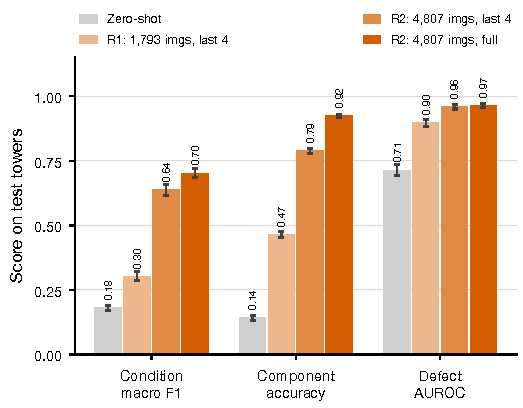
\includegraphics[width=\linewidth]{figs/fig2_finetune.pdf}
\caption{\textbf{More data and a fully trained backbone lift every metric.} Test-tower scores of laya-vision from zero-shot to the round-2 full fine-tune (6,092 images). Whiskers are 95\% bootstrap intervals over images; one training seed per model; no class-share correction.}
\label{fig:finetune}
\end{figure}

Figure~\ref{fig:finetune} and Table~\ref{tab:finetune} show the progression. Round~1 lifts the defect AUROC to 0.898. Its plain accuracy falls because the model learned a training mix with 79\% defects and labels 1,971 of 5,491 good test images as defective. The correction in Eq.~\eqref{eq:prior} raises its condition accuracy from 0.642 to 0.856 and its macro F1 from 0.303 to 0.451. Round~2 adds data, covers all components and has 44\% defects. It improves every metric, and the full model is the best: condition accuracy 0.952 (above the majority answer), macro F1 0.703, component accuracy 0.924, defect AUROC 0.965 and ECE 0.058. For this model the correction changes little (condition accuracy 0.957).

\begin{table}[t]
\centering
\caption{Test-tower results. Images: 6,092 test images. Items: 7,057 ElecVQA-Bench test items. The intervals for laya-vision are in the text and in Fig.~\ref{fig:finetune}. Reference tools are scored on the same items.}
\label{tab:finetune}
\footnotesize
\setlength{\tabcolsep}{4pt}
\begin{tabular}{lcccc}
\toprule
Model & Cond.\ & Comp.\ & Defect & Item \\
 & macro F1 & acc. & AUROC & acc. \\
\midrule
Zero-shot & 0.180 & 0.141 & 0.714 & 0.830 \\
Round 1, last 4 & 0.303 & 0.465 & 0.898 & 0.702 \\
Round 2, last 4 & 0.637 & 0.789 & 0.959 & 0.923 \\
Round 2, full & 0.703 & 0.924 & 0.965 & 0.948 \\
\midrule
ResNet-50, tuned & -- & -- & -- & 0.961 \\
SmolVLM + LoRA & -- & -- & -- & 0.956 \\
SmolVLM, no tuning & -- & -- & -- & 0.830 \\
\bottomrule
\end{tabular}
\end{table}

Per condition, the full model has F1 0.975 for good, 0.710 for rust, 0.826 for corrosion, 0.762 for missing cap and 0.942 for bird nest. Bird nests are always found. Rust has the most false alarms: 152 good images are called rust, so rust precision is 0.62. The 5 test images of other defects are always missed. Among the components, the spacer is the only one that the model does not recognize (recall 0.06, with 18 training images); all other components have a recall of at least 0.87.

On the ElecVQA-Bench items the full model reaches 0.948, below the fine-tuned ResNet-50 (0.961) and SmolVLM with LoRA (0.956). Training takes 24 minutes on an RTX 2080 Ti. The test results remain close to the validation results (condition accuracy 0.952 against 0.935, defect AUROC 0.965 against 0.968), so the model does not overfit the training towers.

\subsection{Latency}\label{sec:latency}

On the RTX 2080 Ti in fp32, one \texttt{predict} call with all four questions takes a median of 72.0\,ms per image (p95 98.5\,ms), including reading and preprocessing the image. The fine-tuned full model takes 74.0\,ms. The condition question alone takes 71.4\,ms, so almost all of the time is spent encoding the image, and further questions are nearly free. With 3.45 key frames per 4\,s segment, as in EVLM~\cite{evlm}, one segment needs 0.25\,s.

We have no Jetson measurement. Scaling by a factor of 9, which we estimated between a GV100-class GPU and a Jetson Orin NX from their fp32 throughput and memory bandwidth, gives about 0.67\,s per image and 2.2\,s per 4\,s segment. On a Jetson Orin, \cite{p2s} measured 2.8\,s per image for SmolVLM-256M and EVLM reports 1.4--6.4\,s per segment~\cite{evlm}, so four answers would take about a quarter of the time of one caption. The comparison is approximate: the hardware differs, and the other systems generate text from video segments, while laya-vision returns labels for single crops.

\subsection{The decision model as a semantic trigger}\label{sec:trigger}

The agenda of~\cite{p2s} calls for hierarchical pipelines in which an inexpensive stage decides which frames reach the VLM, and proposes a detector for this stage. A detector localizes components but does not judge their condition. The decision model does judge the condition, so it can serve as the trigger itself. We use the defect threshold tuned on the validation towers (0.057). On the test towers it passes 931 of 6,092 images (15.3\%) to a following stage and finds 532 of the 601 defects (recall 0.885), with a false-alarm rate of 0.073 among good images and a risk of 179 per 1,000 images, against 987 for always answering good. These rates are computed from the per-image predictions; the cascade itself is not deployed.

\subsection{Calibration and confidence}\label{sec:calib}

After fine-tuning, the defect probability has an ECE of 0.058 (0.178 zero-shot) and an average precision of 0.862, so a mission planner can act on it. The \texttt{judgeable} question, which asks the model whether it can judge the image, is no confidence signal: its AUROC for a correct condition answer is 0.53 zero-shot and 0.31 after fine-tuning. Confidence should come from the calibrated answer probabilities.

\subsection{Federated fine-tuning across drones}\label{sec:fl}

\begin{figure*}[t]
\centering
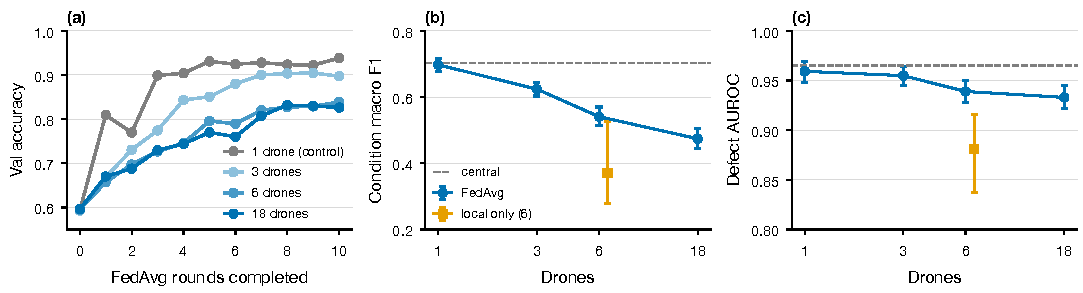
\includegraphics[width=\linewidth]{figs/fig2_federated.pdf}
\caption{\textbf{Splitting the same data over more drones slows FedAvg.} (a) Validation accuracy on 600 images after each round. (b, c) Test-tower condition macro F1 and defect AUROC against the number of drones. FedAvg whiskers are 95\% bootstrap intervals. The local-only marker is the mean of six drone models, and its whisker spans their minimum to maximum. The dashed line is central training. Every run uses the same total training (2.5 passes), with one seed per run.}
\label{fig:federated}
\end{figure*}

\begin{table*}[t]
\centering
\caption{Federated runs on the test towers, with 95\% bootstrap intervals. Local only: mean (minimum--maximum) of the six drone models. Uplink: full-model update in fp16 (229.5\,MB) $\times$ drones $\times$ 10 rounds, calculated, not measured.}
\label{tab:fl}
\footnotesize
\setlength{\tabcolsep}{6pt}
\begin{tabular}{lcccc}
\toprule
Run & Cond.\ macro F1 (95\% interval) & Comp.\ acc. & Defect AUROC & Uplink \\
\midrule
Central (round 2, full) & 0.703 (0.685--0.720) & 0.924 & 0.965 & -- \\
Control, 1 drone & 0.697 (0.677--0.717) & 0.933 & 0.959 & -- \\
FedAvg, 3 drones & 0.624 (0.603--0.643) & 0.874 & 0.955 & 6.9\,GB \\
FedAvg, 6 drones & 0.541 (0.513--0.570) & 0.761 & 0.939 & 13.8\,GB \\
FedAvg, 18 drones & 0.474 (0.444--0.505) & 0.700 & 0.933 & 41.3\,GB \\
Local only, 6 drones & 0.371 (0.278--0.525) & 0.621 & 0.881 & -- \\
\midrule
Server towers, central & 0.558 (0.532--0.584) & 0.894 & 0.903 & -- \\
Fleet FedAvg, base start & 0.513 (0.484--0.540) & 0.593 & 0.932 & 11.5\,GB \\
Fleet FedAvg, fine-tuned start & 0.636 (0.612--0.657) & 0.912 & 0.953 & 11.5\,GB \\
\bottomrule
\end{tabular}
\end{table*}

The control with one drone matches central training: macro F1 0.697 against 0.703 (Table~\ref{tab:fl}). The intervals overlap for all three metrics, so the training loop does not cause the differences below. With the same data spread over more drones, FedAvg loses accuracy (Fig.~\ref{fig:federated}b, c). From 1 to 18 drones, the condition macro F1 falls from 0.697 to 0.474 and the component accuracy from 0.933 to 0.700. The defect AUROC degrades less, from 0.959 to 0.933, so the trigger of Section~\ref{sec:trigger} is the most robust output under federation. The 6- and 18-drone runs are still improving after ten rounds (Fig.~\ref{fig:federated}a), while the control has levelled off; Section~\ref{sec:comm} tests more rounds.

Federation still helps the individual drone. With six drones, FedAvg beats the average drone that trains alone on every metric (macro F1 0.541 against 0.371, defect AUROC 0.939 against 0.881) and the best single drone in defect AUROC (0.939 against 0.916); the best drone's macro F1 (0.525) lies inside the FedAvg interval.

\subsection{A fine-tuned start for the fleet}\label{sec:starts}

The lower part of Table~\ref{tab:fl} compares the two starts on the same fleet. From the published checkpoint, fleet FedAvg reaches a macro F1 of 0.513, a component accuracy of 0.593 and a defect AUROC of 0.932. From the server model it reaches 0.636, 0.912 and 0.953, and the intervals of the two starts do not overlap. The fleet also improves the server model, from 0.558 to 0.636 macro F1 and from 0.903 to 0.953 AUROC, while its images stay on the drones. Its item accuracy (0.937) is close to that of central training on all 18 towers (0.948).

\subsection{What each drone sends}\label{sec:comm}

\begin{figure*}[t]
\centering
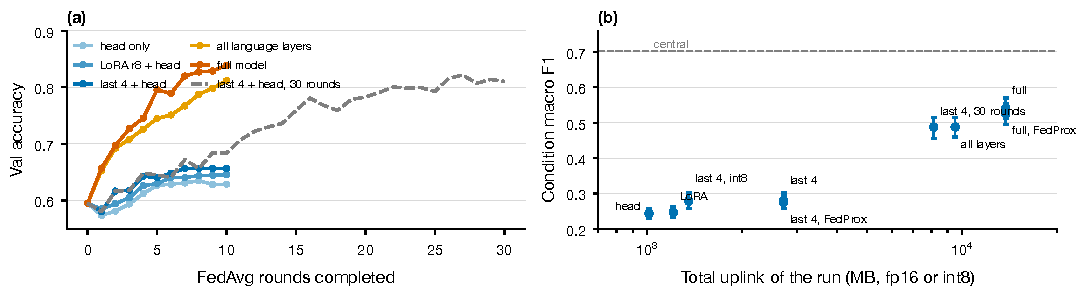
\includegraphics[width=\linewidth]{figs/fig2_roundb.pdf}
\caption{\textbf{From the published checkpoint, small updates learn slowly under FedAvg.} Six tower drones, 10 rounds unless stated. (a) Validation accuracy on 600 images after each round. (b) Test-tower condition macro F1 against the total uplink of the run (update size $\times$ 6 drones $\times$ rounds, calculated); whiskers are 95\% bootstrap intervals; the dashed line is central training of the full model. One seed per run.}
\label{fig:roundb}
\end{figure*}

Each drone sends exactly the part it trains. Table~\ref{tab:parts} lists the size of each choice and its result after 10 FedAvg rounds over six tower drones; the vision encoder (86.4M parameters) is always frozen, and token embeddings make up a quarter of the full update.

\begin{table}[t]
\centering
\caption{Trained and sent part of laya-vision, the size of one drone update (2 bytes per parameter in fp16), and the test result after FedAvg with six tower drones from the published checkpoint (10 rounds, one seed). Central training of the full model: 0.703 and 0.965.}
\label{tab:parts}
\footnotesize
\setlength{\tabcolsep}{3pt}
\begin{tabular}{lcccc}
\toprule
Trained and sent & Params & Update & Macro F1 & AUROC \\
\midrule
Decision head & 8.46M & 16.9\,MB & 0.243 & 0.792 \\
Head + LoRA rank 8 & 10.09M & 20.2\,MB & 0.247 & 0.828 \\
Head + last 4 & 22.62M & 45.2\,MB & 0.281 & 0.838 \\
\quad same, int8 & 22.62M & 22.6\,MB & 0.278 & 0.838 \\
\quad same, FedProx & 22.62M & 45.2\,MB & 0.275 & 0.834 \\
\quad same, 30 rounds & 22.62M & 45.2\,MB & 0.488 & 0.945 \\
Head + 20 layers & 79.27M & 158.5\,MB & 0.488 & 0.931 \\
Full (no vision enc.) & 114.73M & 229.5\,MB & 0.541 & 0.939 \\
\quad same, FedProx & 114.73M & 229.5\,MB & 0.526 & 0.940 \\
\bottomrule
\end{tabular}
\end{table}

From the published checkpoint, the small updates learn little in 10 rounds (Fig.~\ref{fig:roundb}). The head alone reaches a macro F1 of 0.243, LoRA 0.247 and the last four layers 0.281, close to the zero-shot model, while the full update reaches 0.541. Trained centrally, the same last-four update reaches 0.637 (Table~\ref{tab:finetune}), so the small update itself is not the problem. With 30 rounds, the last-four update reaches 0.488 and a defect AUROC of 0.945, and its validation accuracy is still rising (0.66 after 10 rounds, 0.81 after 30). Our reading, supported but not proven, is that averaging six small changes per round moves the shared model slowly, and an update with more parameters moves faster per step.

int8 gives the same result as fp16 (macro F1 0.278 against 0.281, AUROC 0.838 for both), so it halves the uplink for free; FedProx with $\mu=0.01$ changes nothing for either update.

A full-model run needs 6.9--41.3\,GB of uplink and the int8 last-four run 1.4\,GB, against about 0.18\,GB to upload all training images once, so federation keeps images on the drones rather than saving bandwidth.

\subsection{Few labels per drone}\label{sec:labels}

\begin{figure}[t]
\centering
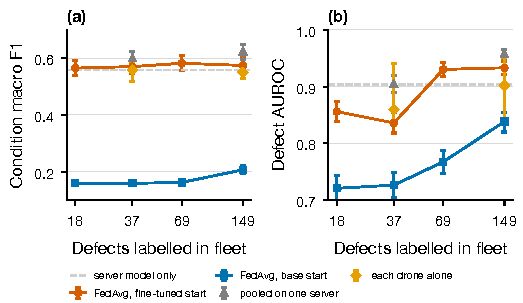
\includegraphics[width=\linewidth]{figs/fig2_roundc.pdf}
\caption{\textbf{Fleet labels help only from the fine-tuned start, and only once the fleet has labelled enough defects.} Five fleet drones with 25, 50, 100 or 200 natural labels each (about 12\% defects), plotted against the number of defects labelled across the fleet; last-four update, 10 rounds. Whiskers: 95\% bootstrap intervals; for drones alone, the range of the five drone models. The dashed line is the server model without fleet labels. One seed per run.}
\label{fig:roundc}
\end{figure}

A real fleet labels few images, and most of them show good components: with 25, 50, 100 and 200 labels per drone, the whole fleet has labelled only 18, 37, 69 and 149 defects. Starting from the published checkpoint, these labels achieve almost nothing; the macro F1 stays between 0.159 and 0.207 (Fig.~\ref{fig:roundc}). Starting from the server model, the macro F1 barely moves, but the defect AUROC follows a U-shape: it first falls below the server model, to 0.856 with 18 labelled defects and 0.836 with 37, and then rises above it, to 0.930 with 69 and 0.933 with 149.

\begin{table}[t]
\centering
\caption{Defect detection with few labels (test towers). Risk, recall and false-alarm rate use the threshold tuned on the validation towers; risk counts 10 per missed defect and 1 per false alarm per 1,000 images; FAR is the false-alarm rate. Drones alone: mean of the five drone models. One seed per run.}
\label{tab:roundc}
\footnotesize
\setlength{\tabcolsep}{3pt}
\begin{tabular}{lccccc}
\toprule
Model & Defects & AUROC & Risk & Recall & FAR \\
\midrule
Server model only & -- & 0.903 & 291 & 0.832 & 0.139 \\
\midrule
FedAvg, tuned start & 18 & 0.856 & 295 & 0.740 & 0.043 \\
 & 37 & 0.836 & 331 & 0.684 & 0.021 \\
 & 69 & 0.930 & 332 & 0.900 & 0.259 \\
 & 149 & 0.933 & 280 & 0.854 & 0.150 \\
\midrule
FedAvg, base start & 18 & 0.721 & 687 & 0.809 & 0.553 \\
 & 149 & 0.838 & 464 & 0.844 & 0.344 \\
\midrule
Pooled centrally & 37 & 0.904 & 211 & 0.832 & 0.050 \\
 & 149 & 0.958 & 181 & 0.870 & 0.059 \\
\midrule
Drones alone (mean) & 37 & 0.860 & 319 & 0.730 & 0.059 \\
 & 149 & 0.902 & 272 & 0.812 & 0.096 \\
\bottomrule
\end{tabular}
\end{table}

Table~\ref{tab:roundc} explains the dip. With few defects, federated averaging makes the model conservative: with 18 labelled defects, the false-alarm rate falls from 0.139 to 0.043 but the defect recall falls from 0.832 to 0.740. The cause is the averaging, not the number of labels. Pooling the same 37 defects on one server keeps the AUROC at the level of the server model (0.904) and lowers the risk to 211, whereas FedAvg over drones that hold between 0 and 15 defects each lowers the AUROC to 0.836. With 149 defects, pooling is still clearly better (AUROC 0.958 against 0.933, risk 181 against 280), but FedAvg now beats the average drone that trains alone (0.933 against 0.902). In this fleet, federated training pays off only once each drone has labelled several defects, about 70 across the fleet.

\subsection{Drones with different image types}\label{sec:hetero}

\begin{figure}[t]
\centering
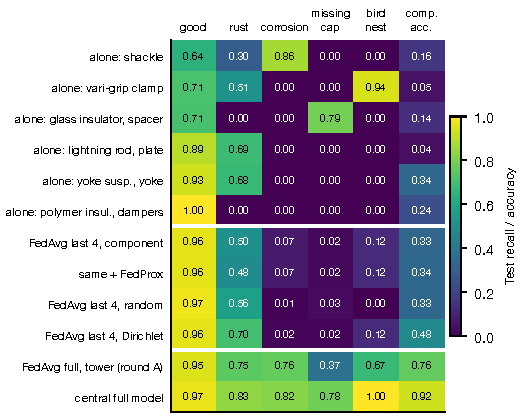
\includegraphics[width=\linewidth]{figs/fig2_roundd.pdf}
\caption{\textbf{Specialist drones learn their own defect type; small-update FedAvg keeps none of them.} Test recall per condition and component accuracy (last column). Top: each drone of the component split trained alone (corrosion exists only on shackles, bird nests only on vari-grip clamps, missing caps only on glass insulators). Middle: FedAvg with the last-four update from the published checkpoint under four splits. Bottom: full-model FedAvg of round~A and central training. One seed per model.}
\label{fig:roundd}
\end{figure}

\begin{table}[t]
\centering
\caption{Drones with different image types: six drones, the 5,107 round-2 images, last-four update from the published checkpoint, 10 rounds. JS: range of the Jensen--Shannon divergence between the condition shares of a drone and of the fleet. Intervals: 95\% bootstrap. One seed per run.}
\label{tab:roundd}
\footnotesize
\setlength{\tabcolsep}{2.5pt}
\begin{tabular}{lcccc}
\toprule
Split & JS & Macro F1 & Comp. & AUROC \\
\midrule
Random & $\le$.002 & .254 (.243--.267) & .334 & .856 \\
Tower & .009--.070 & .281 (.258--.304) & .321 & .838 \\
Component & .128--.333 & .287 (.260--.318) & .331 & .837 \\
\quad + FedProx & .128--.333 & .285 (.259--.317) & .339 & .837 \\
Dirichlet 0.3 & .090--.665 & .291 (.264--.318) & .477 & .833 \\
\quad drones alone & -- & .185 (mean) & .161 & .752 \\
\bottomrule
\end{tabular}
\end{table}

Although the splits differ strongly in how unevenly the conditions are spread over the drones, they give the same macro F1 within their intervals (Table~\ref{tab:roundd}), and FedProx changes nothing. Figure~\ref{fig:roundd} shows why. Each drone that trains alone learns the defect type of its own components well (corrosion 0.86, bird nest 0.94, missing cap 0.79), but FedAvg with the last-four update loses all three types, and it loses them just as much under the random split, where every drone sees every type. The limiting factor is therefore the slow small update, not the differences between drones, and with this update the experiment cannot measure the effect of the split. Full-model FedAvg, in contrast, keeps most of these types (corrosion 0.76, bird nest 0.67, missing cap 0.37). Training alone has its own price: a specialist drone barely recognizes the components of the other drones (component accuracy 0.16 on average, against 0.33 for FedAvg).

\section{Discussion}

\paragraph{What the decision model adds} A large part of the inspection decision does not need a description. From one image encoding, the decision model answers component, defect and condition questions with accuracy close to a fine-tuned describing model, needs no synthetic captions and gives probabilities that can drive a trigger; the describing VLM remains useful for reports and for defects outside the option set.

\begin{figure}[t]
\centering
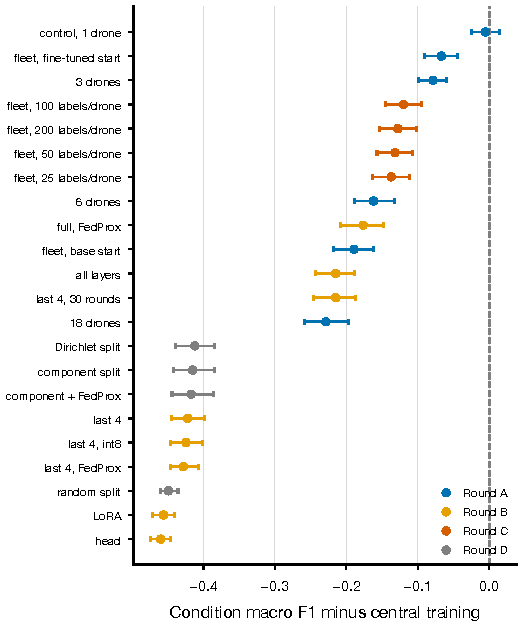
\includegraphics[width=\linewidth]{figs/fig2_overview.pdf}
\caption{\textbf{The cost of federating, across all 22 federated configurations.} Test condition macro F1 minus central training (0.703). Whiskers are each run's 95\% bootstrap interval shifted by the same amount, not an interval of the difference. Rounds C and D use the last-four update; round C starts from the server model. One seed per run.}
\label{fig:overview}
\end{figure}

\paragraph{What federation adds} The collaborative direction of~\cite{p2s} becomes testable once the onboard model is a classifier with a fixed output set. FedAvg across tower-wise drones beats training alone, and a server-fine-tuned start brings the fleet close to central training. Figure~\ref{fig:overview} summarizes all federated runs. The costs are accuracy as the data is split further under a fixed budget, and an uplink of several gigabytes per run for the full model. Small updates cut the uplink and int8 is free, but from the published checkpoint they need many more rounds. The recipe that works throughout is to fine-tune centrally on the data the operator may hold and let the fleet continue; with few labels, federation pays only where the labels cannot be pooled.

\paragraph{Limitations} All configurations have one seed, the drones are simulated on one GPU (uplink is calculated), the Jetson latency is an estimate, and energy is not measured. The data cover one benchmark and one asset type. The update-size and image-type runs start from the published checkpoint, where small updates learn slowly; repeating them from the fine-tuned start, with more seeds and a Jetson measurement, is the next step.

\section{Conclusion}

A 201M-parameter vision-language decision model fails zero-shot on power-line component images, but after fine-tuning on folder labels it reaches 0.948 item accuracy at 74\,ms per image for four questions, with calibrated defect probabilities that can act as a trigger. FedAvg across tower-wise drones beats training alone, and a start fine-tuned on separate server towers brings the fleet close to central training. From the published checkpoint, small updates learn little in ten rounds; int8 halves an update at no measurable cost and FedProx does not help. With 100--200 natural labels per drone (about 70 or more defects in the fleet), fleet FedAvg from the server model improves defect ranking, but less than pooling the same labels; with fewer, it makes the model worse.

\section*{Data and code availability}

The code, the per-image predictions and the evaluation files are in the project repository, branch \texttt{vision-fl} (to be made public on acceptance). ElecVQA-Bench and InsPLAD are public~\cite{elecvqa,insplad}. The laya-vision weights are published under CC BY-NC-SA 4.0~\cite{layavision}.

\section*{Declaration of competing interest}

The author declares no competing interests.

\section*{CRediT authorship contribution statement}

\textbf{Mahdi Khashan:} Conceptualization, Methodology, Software, Investigation, Formal analysis, Writing -- original draft, Writing -- review \& editing.

\section*{Declaration of generative AI use}

During the preparation of this work the author used an AI assistant to write code, analyse results and draft text. The author reviewed and edited the content and takes full responsibility for the publication.

\section*{Acknowledgments}

Experiments in this work were run and tracked with OpenResearch~\cite{openresearch}.

\begin{thebibliography}{99}

\bibitem{p2s} R.~Farahani, N.~Hossein Motlagh, Z.~Azimi, C.~Timmerer, L.~Carnevale, S.~Tarkoma, S.~Dustdar, From pixels to semantics: Edge AI for UAV-based critical infrastructure inspection, arXiv:2609.18448 (2026).

\bibitem{evlm} R.~Farahani, Z.~Azimi, I.~Murturi, A.~Goknil, S.~Sen, C.~Timmerer, S.~Dustdar, EVLM: Intent-driven edge vision language model for UAV-based power line inspection, in: 2026 IEEE International Conference on Edge Computing and Communications (EDGE), 2026. \url{https://doi.org/10.1109/EDGE72783.2026.00014}.

\bibitem{splitvlm} Z.~Azimi, R.~Farahani, S.~Dustdar, C.~Timmerer, Cloud, edge, or split? Profiling onboard and split vision-language model deployment for drone AI, arXiv:2609.25415 (2026).

\bibitem{smolvlm} A.~Marafioti, et al., SmolVLM: Redefining small and efficient multimodal models, arXiv:2504.05299 (2025).

\bibitem{laya} Convai Innovations, Laya, software (2026). \url{https://github.com/NandhaKishorM/laya}.

\bibitem{layavision} Laya Vision, software, commit 9e1e241 (2026). \url{https://github.com/r33drichards/laya-vision}; weights \url{https://huggingface.co/thaitea/laya-vision}.

\bibitem{inarvl} Sabanovic, Maliakel, Brandic, INAR-VL, arXiv:2605.18853 (2026).

\bibitem{guo2017} C.~Guo, G.~Pleiss, Y.~Sun, K.~Q. Weinberger, On calibration of modern neural networks, in: Proceedings of the 34th International Conference on Machine Learning (ICML), 2017.

\bibitem{fedavg} B.~McMahan, E.~Moore, D.~Ramage, S.~Hampson, B.~A. y~Arcas, Communication-efficient learning of deep networks from decentralized data, in: Proceedings of the 20th International Conference on Artificial Intelligence and Statistics (AISTATS), 2017.

\bibitem{zhao2018} Y.~Zhao, M.~Li, L.~Lai, N.~Suda, D.~Civin, V.~Chandra, Federated learning with non-IID data, arXiv:1806.00582 (2018).

\bibitem{fedprox} T.~Li, A.~K. Sahu, M.~Zaheer, M.~Sanjabi, A.~Talwalkar, V.~Smith, Federated optimization in heterogeneous networks, in: Proceedings of Machine Learning and Systems (MLSys), 2020.

\bibitem{flower} D.~J. Beutel, et al., Flower: A friendly federated learning research framework, arXiv:2007.14390 (2020).

\bibitem{fedrouter} Askin, et al., Federate the router, arXiv:2601.22318 (2026).

\bibitem{fedhlm} Solat, Lee, Seif, Niyato, Poor, FedHLM, IEEE Internet of Things Journal (2025). \url{https://doi.org/10.1109/jiot.2025.3618095}.

\bibitem{guardrail} From open-vocabulary detection to structural assessment: An agentic federated approach for guardrail monitoring (2026). \url{https://www.sciencedirect.com/science/article/pii/S2772503026000459}.

\bibitem{elecvqa} ElecVQA-Bench, dataset and code repository (2026). \url{https://github.com/GhostDino/elecvqa-bench}.

\bibitem{insplad} A.~L.~B. Vieira e Silva, et al., InsPLAD: A dataset and benchmark for power line asset inspection in UAV images, International Journal of Remote Sensing (2023). arXiv:2311.01619.

\bibitem{saerens2002} M.~Saerens, P.~Latinne, C.~Decaestecker, Adjusting the outputs of a classifier to new a priori probabilities: A simple procedure, Neural Computation 14 (1) (2002) 21--41.

\bibitem{resnet} K.~He, X.~Zhang, S.~Ren, J.~Sun, Deep residual learning for image recognition, in: IEEE Conference on Computer Vision and Pattern Recognition (CVPR), 2016.

\bibitem{lora} E.~J. Hu, et al., LoRA: Low-rank adaptation of large language models, in: International Conference on Learning Representations (ICLR), 2022.

\bibitem{openresearch} alphaXiv, OpenResearch: The local-first harness and workspace for research agents (2026). \url{https://github.com/alphaXiv/OpenResearch}.

\end{thebibliography}

\end{document}
